\PassOptionsToPackage{table, dvipsnames}{xcolor}
\documentclass[a4paper,twoside,12pt]{toptesi}
\usepackage[T1]{fontenc}
\usepackage[utf8]{inputenc}
\usepackage[italian]{babel}
\usepackage{graphicx}
\usepackage{tikz}
\usetikzlibrary{positioning}
\usepackage{pgfplots}
\usepackage[font=small,skip=1pt]{caption}
\usepackage{xcolor}
\captionsetup[listing]{position=top}
\usepackage{subcaption}

%This equals 1.5 linespacing in Word
\linespread{1.25}

\let\savedlisting\listing
\AtBeginDocument{\let\listing\savedlisting}
\usepackage{listings}
\lstset{
  basicstyle=\ttfamily\footnotesize,
  keywordstyle= \ttfamily\footnotesize
}

\usepackage{bm}


\def\dept{DIPARTIMENTO DI INFORMATICA}
\def\course{CORSO DI LAUREA IN INFORMATICA}
\def\title{Sviluppo e Gestione di Chatbot Addestrati con Tecnica RAG tramite Servizi RESTful}
\def\author{Federico Calò}
\def\relatoreone{Prof.ssa  Berardina Nadja DE CAROLIS}
\def\relatoretwo{}
\def\subject{SISTEMI AD AGENTI}
\def\annoacc{2023 - 2024}
\def\beforecandidate{LAUREANDO:}
\def\beforetitle{TESI DI LAUREA \\ IN \\}
\def\beforeprof{RELATORI:}
\def\beforecorrelatore{CORRELATORI:}
\def\beforeannoacc{ANNO ACCADEMICO}

\makeatletter
\def\cleardoublepage{\clearpage\if@twoside \ifodd\c@page\else
    \hbox{}
    \vspace*{\fill}
    \vspace{\fill}
    \thispagestyle{empty}
    \newpage
    \if@twocolumn\hbox{}\newpage\fi\fi\fi}
\makeatother

\definecolor{codegreen}{rgb}{0,0.6,0}
\definecolor{codegray}{rgb}{0.5,0.5,0.5}
\definecolor{codepurple}{rgb}{0.19, 0.55, 0.91}
\definecolor{backcolour}{rgb}{1.0, 0.98, 0.98}

\lstdefinestyle{mystyle}{
    backgroundcolor=\color{backcolour},   
    commentstyle=\color{codegreen},
    keywordstyle=\color{codepurple},
    numberstyle=\tiny\color{codegray},
    stringstyle=\color{codepurple},
    basicstyle=\ttfamily\footnotesize,
    breakatwhitespace=false,         
    breaklines=true,                 
    captionpos=b,                    
    keepspaces=true,                 
    numbers=left,                    
    numbersep=5pt,                  
    showspaces=false,                
    showstringspaces=false,
    showtabs=false,                  
    tabsize=2
}
\lstset{style=mystyle}
\setlength{\parindent}{0pt}
\setlength{\parskip}{5pt}
\usepackage{hyperref}
\hypersetup{
    colorlinks = true,
    allcolors=black
}

\newcommand{\boldtt}[1]{\textbf{\texttt{#1}}}

\begin{document}

\begin{titlepage}
	\begin{tikzpicture}[remember picture,overlay]
		\centering
		\node[yshift=-6 cm] (logo) at (current page.north) {
\includegraphics[width=0.75\linewidth]{immagini/uniba.jpg}};
			\node[text width=50em,yshift=0.25cm, align = center, below = of logo](dipartimento){\normalsize \dept};
			\node[text width=40em, align = center, yshift=.55cm,below = of dipartimento](course){\normalsize \course};
		\node[text width=35em,align = center,  yshift=1.2cm,below = of course](line){\par\noindent\rule{\textwidth}{0.4pt}};
		\node[text width=40em, align = center, yshift=.55cm,below = of line](lia){\normalsize \beforetitle \xspace \subject };
		
  \node[text width=40em, align = center, yshift=-0.5cm,below = of lia](title){\bfseries \parbox{12cm}{\fontsize{21pt}{20pt}\selectfont \centering \title\par}};
  
	\node[text width=35em, align = left, yshift=-1cm,below = of title](relatoretit){\normalsize \textbf{\beforeprof} };
 	\node[text width=35em, align = left, yshift=1cm,below = of relatoretit](relatore){\large \relatoreone \\ \relatoretwo};


      
		\node[text width=35em, align = right, yshift=-1cm,below = of title](candidatetit){\normalsize \textbf{\beforecandidate}};
		 \node[text width=35em, align = right, yshift=1cm,below = of candidatetit](candidate){\large \author};


  \node[text width=35em,align = center,  yshift= -3cm,below = of candidate](line2){\par\noindent\rule{\textwidth}{0.4pt}};
	
  
  \node[text width=50em, align = center, yshift=0.5cm,below = of line2](year){\large \beforeannoacc\xspace \annoacc};
	\end{tikzpicture}
\end{titlepage}


\cleardoublepage


\pagenumbering{roman}

\tableofcontents

\cleardoublepage

\pagenumbering{arabic}
\setcounter{page}{1}
\addcontentsline{toc}{chapter}{Introduzione}

\chapter*{Introduzione}
Nel contesto odierno, caratterizzato da una crescente interazione tra utenti e sistemi digitali, i chatbot stanno emergendo come strumenti fondamentali per migliorare l'esperienza dell'utente e ottimizzare i processi aziendali. Tuttavia, la creazione e gestione di chatbot avanzati richiede un approccio integrato che sfrutti le migliori tecniche di addestramento e architetture software.

Questa tesi si propone di affrontare tale sfida attraverso la progettazione e realizzazione di un ecosistema avanzato per la creazione e gestione di chatbot. L'obiettivo principale del progetto è sviluppare una piattaforma che consenta la creazione di diversi chatbot addestrati utilizzando la metodologia Retrieval-Augmented Generation (RAG), i quali possono interfaccirsi tra loro e con l'utente attraverso servizi REST.

Per garantire una fruizione ottimale e una gestione efficiente dei chatbot, è stata progettata una soluzione integrata che comprende:
\begin{itemize}
\item \textbf{Frontend in ReactJS}: Un'interfaccia utente interattiva e dinamica che facilita l'interazione degli utenti con i chatbot. ReactJS è stato scelto per la sua capacità di creare applicazioni web veloci e reattive.

\item \textbf{Servizi REST}: Interfacce di programmazione che permettono la comunicazione tra il frontend, i servizi backend e i vari bot. Le API sono state sviluppate utilizzando due tecnologie complementari: Spring Boot e Python.

\item \textbf{Bot RAG}: L'approccio Retrieval-Augmented Generation è stato adottato per addestrare i chatbot, sviluppati in Python, combinando tecniche di recupero di informazioni e generazione di risposte, al fine di migliorare la pertinenza e l'accuratezza delle risposte fornite dai bot.
\end{itemize}
La realizzazione di questo ecosistema richiede un'integrazione armoniosa di componenti software e tecniche di machine learning, mirata a offrire una piattaforma versatile e potente per lo sviluppo di chatbot avanzati. L'importanza di questo progetto risiede nella sua capacità di semplificare la creazione e gestione di chatbot sofisticati, migliorando significativamente l'interazione uomo-macchina e offrendo soluzioni scalabili per diverse applicazioni aziendali e di consumo.


\chapter{Intrroduzione ai LLMs e ai servizi REST}

I Large Language Models (LLMs) rappresentano una classe avanzata di modelli di intelligenza artificiale progettati per comprendere, generare e interagire con il linguaggio umano a livelli di complessità senza precedenti. Questi modelli sono stati all’avanguardia delle ricerche nel campo del Natural Language Processing (NLP) e sono stati progettati per comprendere, interpretare, generare e tradurre testi in linguaggio naturale. La loro "grandezza"(large) non deriva solo dalla dimensione del modello in termini di numero di parametri, ma anche dall’enrome quantità di dati su cui vengono addestrati. Questi modelli apprendono autonomamente le strutture linguistiche e le relazioni semantiche dai dati, permettendo loro di generare testi coerenti e pertinenti, rispondere a domande, riassumere documenti e molto altro.

I servizi RESTful (Representational State Transfer) rappresentano un'architettura per la creazione di applicazioni web e API che consente una comunicazione semplice ed efficiente tra client e server. Basati sui principi dell'architettura REST, questi servizi utilizzano il protocollo HTTP per gestire le richieste e le risposte tra le diverse componenti di un sistema, fornendo quindi un modo standardizzato e scalabile per la comunicazione tra queste parti. Essi giocano un ruolo cruciale nella connessione tra il frontend e il backend di sistemi complessi, come quelli che utilizzano modelli di linguaggio avanzati. Per esempio, nel contesto di un chatbot addestrato con la metodologia RAG, i servizi RESTful possono facilitare la comunicazione tra l'interfaccia utente (frontend) e i servizi di elaborazione e generazione del linguaggio (backend), garantendo un'interazione fluida e reattiva.

Si vedrà in seguito come si sono combinate queste due tecniche di programmazione, il potenziale attuale e i futuri sviluppi.

\section{Storia e caratteristiche degli LLMs}
Il viaggio dei Large Language Models (LLMs) inizia negli anni ’50, quando l'intelligenza artificiale era ancora agli albori. In quei primi giorni, i ricercatori si concentravano principalmente su sistemi basati su regole e approcci simbolici. I modelli di linguaggio dell'epoca erano piuttosto rudimentali e si basavano su semplici regole predefinite, senza la capacità di apprendere direttamente dai dati.

Con l'avvento del machine learning negli anni '80 e '90, le cose iniziarono a cambiare. I modelli statistici, come i modelli di Markov nascosti e gli n-grammi, iniziarono a essere utilizzati per l'elaborazione del linguaggio naturale (NLP). Sebbene questi modelli offrissero un miglioramento rispetto ai sistemi basati su regole, erano ancora limitati nella loro capacità di comprendere e generare linguaggio naturale in modo complesso.

La vera rivoluzione arrivò con l'introduzione delle reti neurali e del deep learning nei primi anni 2000. Architetture come le reti neurali ricorrenti (RNN) e le LSTM (Long Short-Term Memory) iniziarono a gestire meglio le sequenze di testo e le dipendenze a lungo termine, portando a progressi significativi nella NLP.

Ma è stato il 2017 a segnare una svolta decisiva con l'introduzione dell'architettura dei trasformatori nel paper "Attention is All You Need" di Vaswani et al. Questa innovazione ha rivoluzionato il campo, aprendo la strada a modelli come BERT (Bidirectional Encoder Representations from Transformers) e GPT (Generative Pre-trained Transformer). Questi modelli hanno dimostrato capacità straordinarie nella gestione del linguaggio, grazie alla loro abilità di catturare contesti complessi e gestire grandi quantità di dati.

Negli ultimi anni, i LLMs hanno raggiunto nuove vette con modelli di enormi dimensioni come GPT-3 e GPT-4. Questi modelli, con i loro miliardi di parametri, sono stati addestrati su enormi corpus di dati, permettendo loro di comprendere e generare testo con una precisione e coerenza senza precedenti.

Le caratteristiche distintive dei LLMs sono davvero notevoli. Innanzitutto, la loro grandezza è impressionante: modelli come GPT-3 hanno 175 miliardi di parametri, una quantità enorme che consente di catturare e rappresentare una vasta gamma di conoscenze linguistiche e semantiche. Questo grande numero di parametri è fondamentale per permettere ai modelli di comprendere e generare testo in modo accurato e fluido.

Inoltre, gli LLMs sono addestrati su enormi dataset provenienti da una varietà di fonti, tra cui libri, articoli e conversazioni online. Questo ampio addestramento consente ai modelli di apprendere un'ampia gamma di stili e contenuti linguistici.

Una delle caratteristiche più avanzate è la loro capacità di comprensione e generazione del linguaggio. Gli LLMs non solo comprendono il contesto delle conversazioni e dei testi, ma possono anche generare risposte pertinenti e coerenti, eseguire traduzioni, riassumere documenti e persino creare testi originali.

I LLMs utilizzano tecniche di apprendimento non supervisionato e pre-addestramento per costruire una base solida di conoscenze linguistiche. Questo approccio consente ai modelli di acquisire una comprensione generale del linguaggio prima di essere affinati su compiti specifici, migliorando ulteriormente la loro capacità di applicarsi a vari compiti di NLP.

Infine, l'architettura dei trasformatori, alla base della maggior parte degli LLMs moderni, è fondamentale. I trasformatori utilizzano meccanismi di attenzione per pesare l'importanza delle diverse parti del testo, gestendo in modo più efficace le dipendenze a lungo termine e migliorando la comprensione del contesto.

In sintesi, i Large Language Models hanno rappresentato una delle più grandi innovazioni nell'ambito dell'intelligenza artificiale. La loro evoluzione ha trasformato il modo in cui interagiamo con il linguaggio e ha aperto nuove possibilità per applicazioni in vari ambiti, dall'assistenza clienti alla generazione di contenuti creativi.

\subsection{Applicazioni degli LLM}

I Large Language Models (LLMs) hanno trasformato radicalmente il campo dell'intelligenza artificiale e dell'elaborazione del linguaggio naturale (NLP), aprendo nuove possibilità applicative in vari settori. Questi modelli, grazie alla loro capacità di comprendere e generare testo con una precisione senza precedenti, sono diventati strumenti essenziali per una vasta gamma di applicazioni.

Una delle principali applicazioni degli LLMs è nei sistemi di assistenza virtuale. Tecnologie come Siri, Alexa e Google Assistant utilizzano LLMs per comprendere e rispondere alle richieste degli utenti, eseguire comandi vocali, fornire informazioni in tempo reale e interagire con altre applicazioni. Questi assistenti virtuali si basano sulla capacità dei LLMs di interpretare il linguaggio naturale, comprendere il contesto e generare risposte appropriate in modo fluido e naturale.

Nel settore della generazione di contenuti, i LLMs vengono utilizzati per creare testi automaticamente. Ad esempio, possono generare articoli di notizie, post sui social media, descrizioni di prodotti, e persino testi creativi come poesie o storie. Strumenti come GPT-3 hanno dimostrato di poter produrre contenuti di alta qualità che sono quasi indistinguibili da quelli scritti da esseri umani, accelerando il processo di creazione di contenuti e rendendolo più accessibile.

Gli LLMs sono anche ampiamente utilizzati nei sistemi di traduzione automatica. Modelli come quelli implementati da Google Translate e altri servizi di traduzione online sono in grado di tradurre testi da una lingua all'altra con una precisione e fluidità sempre maggiori. Questi modelli sfruttano la loro comprensione approfondita delle strutture linguistiche e delle relazioni semantiche per produrre traduzioni che rispettano il contesto e il significato originale.

Nel campo della analisi del sentiment e del monitoraggio dei social media, i LLMs vengono utilizzati per analizzare grandi volumi di dati testuali, come post sui social media, recensioni dei clienti e articoli di opinione, per comprendere l'opinione pubblica e il sentiment generale riguardo a prodotti, marchi o eventi. Questa analisi permette alle aziende di monitorare la percezione del pubblico e di prendere decisioni informate basate sui feedback raccolti.

Un'altra applicazione emergente degli LLMs è nel supporto alla scrittura e alla ricerca. Strumenti come quelli sviluppati da OpenAI vengono utilizzati per assistere scrittori, ricercatori e studenti nel creare bozze, riassumere articoli, generare idee o formulare risposte a domande complesse. Questi modelli possono accelerare il processo creativo e migliorare la produttività, fornendo suggerimenti pertinenti e contenuti coerenti in tempo reale.

Infine, gli LLMs trovano applicazione anche nel supporto decisionale aziendale. Attraverso l'analisi di dati testuali e documenti, questi modelli possono aiutare le aziende a estrarre informazioni critiche, fare previsioni basate su trend emergenti e supportare la presa di decisioni strategiche. Questo è particolarmente utile in contesti come l'analisi di mercato, la gestione del rischio e la pianificazione aziendale.


\section{Storia e caratteristiche dei servizi REST}

Nel panorama attuale dello sviluppo software, i servizi RESTful hanno acquisito un ruolo fondamentale grazie alla loro semplicità ed efficacia nel facilitare la comunicazione tra diverse applicazioni e componenti di un sistema. L'architettura REST, acronimo di Representational State Transfer, è stata introdotta da Roy Fielding nel 2000 e ha rapidamente rivoluzionato il modo in cui le applicazioni web sono progettate e sviluppate.

Un aspetto chiave dei servizi RESTful è la loro natura stateless. Questo significa che ogni richiesta effettuata dal client verso il server è indipendente dalle altre; il server non conserva informazioni sullo stato delle richieste precedenti. Questa caratteristica semplifica notevolmente la scalabilità delle applicazioni, poiché non è necessario che il server gestisca sessioni o mantenga traccia delle interazioni passate. Ogni richiesta contiene tutte le informazioni necessarie per essere processata in modo autonomo.

La separazione tra client e server è un altro principio cardine di REST. In questa architettura, il client è responsabile della presentazione e dell'interfaccia utente, mentre il server gestisce la logica di business e l'archiviazione dei dati. Questo tipo di suddivisione permette uno sviluppo più modulare, in cui le componenti del frontend e del backend possono evolvere in modo indipendente. Ad esempio, è possibile aggiornare l'interfaccia utente senza dover necessariamente intervenire sulla logica del server, e viceversa.

Un'altra caratteristica distintiva dei servizi RESTful è l'utilizzo di un'interfaccia uniforme per la comunicazione. I metodi standard del protocollo HTTP, come GET, POST, PUT e DELETE, sono utilizzati per eseguire operazioni su risorse identificate da URL specifici. Questo approccio non solo semplifica lo sviluppo, ma rende anche le API RESTful facili da comprendere e utilizzare, poiché seguono convenzioni ben definite e universalmente riconosciute.

Le risorse, in un'architettura RESTful, sono rappresentate tramite URL. Ogni risorsa, che può essere un oggetto, un servizio, o una qualsiasi entità gestita dal server, è accessibile tramite un URL univoco. Questo rende l'accesso e la manipolazione delle risorse intuitivi e facilmente gestibili, poiché tutto è strutturato attorno a un sistema di indirizzamento chiaro e organizzato.

Un ulteriore vantaggio offerto dai servizi RESTful è la possibilità di caching. Le risposte alle richieste possono essere memorizzate dal client per un certo periodo di tempo, riducendo così la necessità di ripetere richieste identiche e migliorando l'efficienza complessiva del sistema. Il caching permette di alleviare il carico sui server e di velocizzare l'accesso ai dati, migliorando l'esperienza utente.

Infine, l'architettura REST supporta la realizzazione di sistemi stratificati. Ciò significa che tra il client e il server possono essere introdotti vari componenti intermediari, come proxy e gateway, che svolgono funzioni aggiuntive come la gestione della sicurezza, il bilanciamento del carico e l'ottimizzazione delle prestazioni. Questa stratificazione permette di scalare il sistema in modo più efficiente e di aggiungere nuove funzionalità senza interrompere l'intera infrastruttura.

Nel complesso, i servizi RESTful hanno rivoluzionato il modo in cui le applicazioni web e mobile interagiscono con il backend. La loro semplicità, combinata con una grande flessibilità, li rende ideali per la costruzione di sistemi complessi e distribuiti, come i microservizi, che possono essere sviluppati, testati e aggiornati indipendentemente. La diffusione di questa architettura ha consentito lo sviluppo di applicazioni altamente scalabili e manutenibili, in grado di adattarsi rapidamente alle esigenze in continua evoluzione del mondo digitale.

\subsection{Applicazioni dei servizi REST}

I servizi RESTful hanno trovato un'ampia applicazione in numerosi settori e tipologie di sistemi, grazie alla loro flessibilità, semplicità e capacità di facilitare l'integrazione tra diverse componenti software. L'approccio REST è diventato lo standard de facto per la progettazione di API (Application Programming Interface), utilizzate per collegare diverse applicazioni, servizi e dispositivi in modo efficiente e scalabile.

Una delle applicazioni più comuni dei servizi REST è nello sviluppo di applicazioni web e mobile. Le API RESTful consentono a queste applicazioni di comunicare con il backend per recuperare dati, inviare informazioni e interagire con altri servizi. Ad esempio, un'app mobile di social media utilizza REST per caricare i feed degli utenti, pubblicare nuovi post, gestire notifiche e interagire con altre funzionalità della piattaforma. La natura stateless di REST rende possibile gestire un elevato numero di richieste simultanee, rendendo le applicazioni più rapide e reattive.

I servizi RESTful sono anche ampiamente utilizzati nei microservizi, un'architettura che scompone le applicazioni in una serie di piccoli servizi indipendenti, ciascuno dei quali svolge una funzione specifica. Questa struttura permette di sviluppare, distribuire e scalare i componenti in modo indipendente, riducendo la complessità e migliorando l'agilità del sistema. In questo contesto, REST funge da collante che permette ai vari microservizi di comunicare tra loro in modo standardizzato e coerente.

Nel campo dell'Internet of Things (IoT), REST viene spesso impiegato per facilitare la comunicazione tra dispositivi intelligenti e i sistemi backend che li gestiscono. Ad esempio, i dispositivi IoT, come termostati intelligenti o sistemi di monitoraggio remoto, utilizzano API RESTful per inviare dati sensoriali a un server centrale, che li elabora e restituisce comandi o configurazioni aggiornate. La leggerezza e la scalabilità di REST lo rendono ideale per gestire reti di dispositivi distribuiti e a bassa potenza.

Anche nel settore delle integrazioni tra sistemi eterogenei, i servizi RESTful sono ampiamente utilizzati. Grazie alla loro natura universale e indipendente dalla piattaforma, REST permette a sistemi sviluppati con tecnologie diverse di comunicare tra loro. Ad esempio, un sistema di gestione delle risorse umane potrebbe utilizzare REST per sincronizzare dati con un sistema di contabilità o con applicazioni di terze parti per la gestione dei salari.

Infine, REST è largamente impiegato nella creazione di applicazioni cloud. I servizi cloud come AWS, Google Cloud e Microsoft Azure offrono API RESTful per gestire risorse cloud, come server, database e servizi di storage. Queste API permettono agli sviluppatori di automatizzare la gestione delle risorse cloud, implementando funzioni di scalabilità automatica, monitoraggio delle performance e gestione delle configurazioni.

\section{Servizi REST e LLMs}

L'interazione tra servizi RESTful e Large Language Models (LLMs) rappresenta un approccio potente e versatile per sfruttare le capacità avanzate dell'intelligenza artificiale in applicazioni web e mobile. I servizi REST, grazie alla loro natura semplice e standardizzata, forniscono un'infrastruttura ideale per orchestrare e gestire la comunicazione tra i client e i modelli di intelligenza artificiale, come gli LLMs, che sono in grado di comprendere e generare linguaggio naturale.

In un'architettura in cui i servizi RESTful fungono da intermediari tra l'interfaccia utente e i LLMs, ogni richiesta effettuata dal client può essere facilmente instradata verso il modello AI appropriato per l'elaborazione. Ad esempio, un utente potrebbe inviare una domanda o un comando tramite un'applicazione web o mobile. Questa richiesta viene trasmessa tramite una chiamata API RESTful al server, dove i servizi REST gestiscono la richiesta e la inoltrano all'LLM per l'elaborazione.

Uno dei principali vantaggi dell'utilizzo di servizi REST in combinazione con LLMs è la loro capacità di gestire richieste stateless. Questo significa che ogni richiesta inviata al server è indipendente e contiene tutte le informazioni necessarie per essere elaborata. Gli LLMs, che possono richiedere risorse computazionali significative, possono così concentrarsi sull'elaborazione del linguaggio naturale senza doversi preoccupare dello stato della sessione utente. Questo approccio semplifica l'infrastruttura e migliora la scalabilità del sistema.

Un'altra area in cui i servizi REST possono migliorare l'integrazione con gli LLMs è attraverso la modularità. I servizi RESTful possono essere progettati per svolgere funzioni specifiche, come l'autenticazione, la gestione delle richieste, o l'elaborazione di dati prima o dopo l'intervento degli LLMs. Questa modularità consente di creare pipeline di elaborazione flessibili, in cui diverse componenti possono essere aggiornate o sostituite senza interrompere l'intero sistema. Per esempio, è possibile implementare un servizio REST che pre-processa i dati dell'utente, rendendoli più facilmente comprensibili per l'LLM, migliorando così la precisione delle risposte generate.

Inoltre, i servizi RESTful possono facilitare l'integrazione di LLMs con altre risorse e servizi. Ad esempio, un'API REST può essere utilizzata per recuperare dati da un database o da una fonte esterna, che poi vengono combinati con le capacità generative dell'LLM per fornire risposte più complete e contestuali. Questo approccio, noto come Retrieval-Augmented Generation (RAG), permette agli LLMs di accedere a informazioni specifiche e aggiornate, migliorando significativamente la qualità delle risposte.

Infine, i servizi RESTful sono particolarmente adatti per automatizzare e scalare l'uso degli LLMs in applicazioni distribuite. Grazie alla loro compatibilità con il protocollo HTTP e la loro facilità di implementazione, i servizi REST possono essere utilizzati per orchestrare l'elaborazione di grandi volumi di richieste simultanee, bilanciando il carico tra diversi istanze dell'LLM e garantendo che le risposte siano fornite in tempi rapidi. Questo è cruciale per applicazioni come i chatbot su larga scala, dove l'interazione in tempo reale con gli utenti è essenziale.

In sintesi, l'integrazione di LLMs con servizi RESTful offre una soluzione potente e flessibile per implementare capacità avanzate di elaborazione del linguaggio naturale in applicazioni moderne. Grazie alla loro modularità, scalabilità e facilità di integrazione, i servizi RESTful non solo facilitano la comunicazione con i modelli di intelligenza artificiale, ma permettono anche di sfruttare appieno le loro potenzialità in un'ampia gamma di scenari applicativi.


\chapter{Analisi e progettazione}

Il progetto nasce dall'idea di sviluppare un sistema di chatbot avanzati, addestrati su argomenti specifici utilizzando la tecnica RAG (Retrieval-Augmented Generation) applicata a file PDF, con interazione attraverso servizi RESTful. Durante le fasi di analisi e progettazione, è stata adottata un'architettura a microservizi, implementata con Spring Boot, un framework Java, e Python, scelto per la sua vasta gamma di librerie dedicate all'addestramento di modelli conversazionali. L'obiettivo principale del progetto è creare una piattaforma scalabile, modulare e facilmente integrabile in sistemi complessi, garantendo semplicità di gestione e manutenzione.

Un esempio applicativo del sistema è in ambito sanitario, dove ogni reparto di una struttura potrebbe disporre di un chatbot specificamente addestrato sui documenti PDF forniti dai medici del reparto stesso. I vari bot sarebbero accessibili tramite un'interfaccia grafica condivisa, che consentirebbe ai medici di consultare il chatbot del proprio reparto o di altri reparti per ottenere informazioni non presenti nei propri archivi, facilitando così la collaborazione inter-disciplinare.

\begin{center}

\fbox{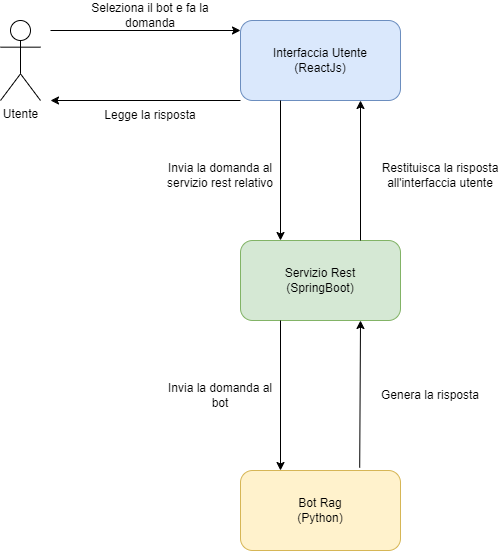
\includegraphics[width=0.8\textwidth, height=0.8\textheight, keepaspectratio]{immagini/1.png}}

\end{center}

\section{Stack tecnologico}

Ogni bot si basa su queste tecnologie:

\begin{itemize}
	\item SpringBoot
	\item Python
	\item LangChain
	\item Ollama
\end{itemize} 

Spring Boot è utilizzato per lo sviluppo dei servizi RESTful che costituiscono il cuore del backend del sistema. Questa potente piattaforma Java semplifica la creazione di applicazioni stand-alone e basate su microservizi. Spring Boot consente di costruire API REST robuste e scalabili, gestendo in modo efficiente le comunicazioni tra il frontend e i vari componenti del backend, e garantendo un'architettura modulare e facilmente estendibile.

Python, infine, è impiegato per la creazione e l'addestramento dei bot. Conosciuto per la sua sintassi chiara e la vasta gamma di librerie specializzate, Python è particolarmente adatto per il machine learning e l'elaborazione del linguaggio naturale. Le librerie di Python, come TensorFlow e PyTorch, permettono di sviluppare modelli avanzati per i bot, che possono essere addestrati per rispondere in modo preciso e contestuale alle esigenze degli utenti.

LangChain è un framework a supporto di Python per la vettorizzazione dei documenti sui quali si desidera addestrare il bot, per la tokenizzazione della domande dell'utente e il calcolo del coefficente di similarità tra la tokenizzazione della domanda e la tokenizzazione dei documenti. LangChain si coordina con Ollama, software per il download e l'avvio di LLM in locale.

La relazione tra queste tecnologie può essere rappresentata in modo chiaro ed efficace attraverso il seguente schema:
\begin{center}

\fbox{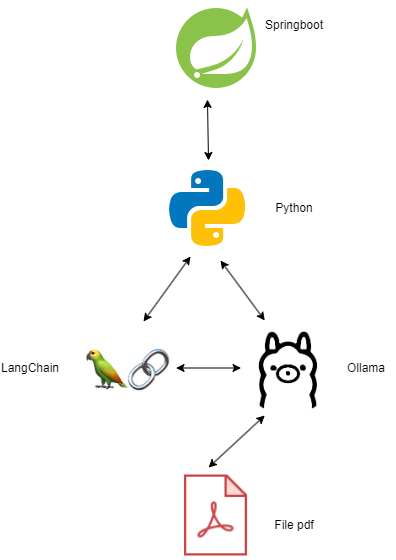
\includegraphics[width=0.42\textwidth, height=0.7\textheight, keepaspectratio]{immagini/3.png}}

\end{center}

Ollama permette di scaricare e utilizzare localmente il modello linguistico (LLM) desiderato, offrendo una soluzione che coniuga efficienza e sicurezza. Questa tecnologia consente di eseguire l'intero programma direttamente su un server locale, eliminando la necessità di trasferire dati sensibili verso piattaforme cloud esterne. Grazie a questa architettura, è possibile conservare i file PDF e altri dati critici in un ambiente controllato, riducendo al minimo i rischi di accessi non autorizzati o violazioni della privacy.

Oltre a garantire una maggiore protezione dei dati, l'approccio locale contribuisce a ridurre i costi operativi legati all'infrastruttura. L'assenza di dipendenze da servizi cloud esterni non solo abbatte i costi ricorrenti di archiviazione e calcolo, ma aumenta anche l'autonomia nella gestione del sistema, semplificando il controllo delle risorse hardware e software. Questa configurazione è particolarmente vantaggiosa per aziende e organizzazioni che devono trattare dati sensibili o rispettare rigorosi requisiti di conformità normativa.


\begin{center}

\fbox{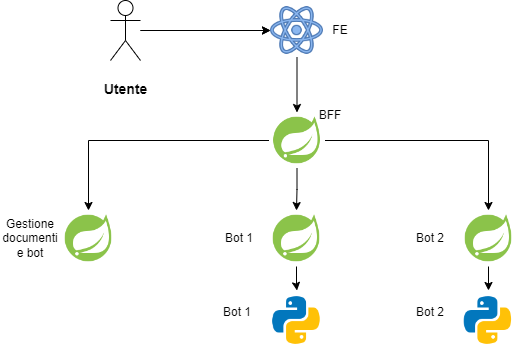
\includegraphics[width=0.8\textwidth, height=0.8\textheight, keepaspectratio]{immagini/2.png}}
\end{center}

In un'infrastruttura complessa composta da più bot che operano contemporaneamente, l'orchestrazione del sistema può essere organizzata in modo chiaro e modulare. Ciascun bot è costituito da due componenti principali: un progetto Python, che si occupa dell'addestramento e dell'interrogazione del modello linguistico (LLM) sui relativi file PDF, e un servizio Spring Boot, che funge da ponte per consentire al bot di comunicare con il resto dell'applicativo.

A supporto di questa struttura, esiste un progetto Spring Boot separato, dedicato alla gestione del caricamento dei documenti per ogni bot. Questo servizio è inoltre responsabile della registrazione dei bot nel database, garantendo un'integrazione coerente e centralizzata delle varie istanze operative.

Per completare l'infrastruttura, un ulteriore progetto Spring Boot è implementato come Backend For Frontend (BFF), che funge da intermediario tra un eventuale frontend e l'intero backend. Questa soluzione facilita le interazioni, offrendo un punto di accesso unico e semplificando la comunicazione tra le varie componenti del sistema.

Questa configurazione modulare non solo rende l'infrastruttura facilmente scalabile, consentendo l'aggiunta di nuovi bot, ma garantisce anche una gestione efficiente e una comunicazione fluida tra le diverse parti dell'ecosistema.

\subsection{Creazione e addestramento dei chatbot}

Nell'infrastruttura creata, ogni volta che è necessario sviluppare e addestrare un nuovo chatbot su documenti PDF specifici di una determinata tematica, viene creato un progetto in Python che utilizza quattro librerie chiave:

\begin{itemize}
	\item Flask: Questa libreria consente di creare endpoint REST, facilitando la comunicazione tra il chatbot e l'applicazione backend basata su Spring Boot tramite il protocollo REST.
	\item LangChain e Chroma: Queste librerie sono responsabili della vettorizzazione dei documenti PDF e del recupero delle informazioni rilevanti in risposta ai prompt inseriti dagli utenti attraverso l'interfaccia grafica.
	\item Ollama: Permette l'interazione tra il programma e il modello di LLM (Large Language Model) installato localmente, gestendo le richieste e le risposte del chatbot.
\end{itemize}

Parallelamente, viene avviato un progetto in Spring Boot per gestire la comunicazione tra il chatbot e l'interfaccia grafica tramite il protocollo REST, garantendo un'integrazione fluida e coerente tra il frontend e il backend.

\begin{lstlisting}[language=Python, caption=Microservizi Python]
@app.route('/message', methods=['POST'])
def botAlimentazioneMessage():
    jsonContent = request.json
    query = jsonContent.get('query')
    print(f"Query: {query}")

    response = llm.invoke(query)
    responseAnswer = {"message": check_and_translate(response)}

    return responseAnswer


@app.route('/load-pdf', methods=['POST'])
def loadPdf():
    file = request.files['file']
    fileName = file.filename
    saveFile = ""
    if os.name == 'nt':
        saveFile = pathAddestramento + "\\" + fileName
    else:
        saveFile = pathAddestramento + "/" + fileName
    file.save(saveFile)
    print(f"File salvato: {saveFile}")

    if not fileName[-4:] == ".pdf":
        response = {
            "status": "success",
            "fileName": fileName,
            "docLen": 0,
            "chunks": 0
        }
        return response

    loadPdf = PDFPlumberLoader(saveFile)

    docs = loadPdf.load_and_split()
    print(f"Doc len: {len(docs)}")

    chunks = text_splitter.split_documents(docs)
    print(f"Doc len: {len(chunks)}")

    response = {
        "status": "success",
        "fileName": fileName,
        "docLen": len(docs),
        "chunks": len(chunks)
    }
    if(len(docs)==0 or len(chunks)==0 ):
        response = {
            "status": "failed",
            "fileName": fileName,
            "docLen": len(docs),
            "chunks": len(chunks)
        }
    else:
        vectorStore = Chroma.from_documents(documents=chunks, embedding=embedding, persist_directory=pathAddestramento)
        vectorStore.persist()
    return response


@app.route('/message-pdf', methods=['POST'])
def askPdf():
    jsonContent = request.json
    query = jsonContent.get('query')
    print(f"Query: {query}")

    print(f"Carico il VectorStore")
    vectorStore = Chroma(persist_directory=pathAddestramento,
                         embedding_function=embedding)

    print(f"Creo la chain")
    retriever = vectorStore.as_retriever(
        search_type="similarity_score_threshold",
        search_kwargs={
            "k": 20,
            "score_threshold": 0.3,
        },
    )

    document_chain = create_stuff_documents_chain(llm, rawPrompt)
    chain = create_retrieval_chain(retriever, document_chain)

    result = chain.invoke({"input": f"Rispondi in italiano: {query}"})

    print(result)

    sources = []
    for doc in result["context"]:
        sources.append(
            {"source": doc.metadata["source"], "pageContent": doc.page_content}
        )

    responseAnswer = {"answer": check_and_translate(result["answer"]), "sources": sources}

    return responseAnswer


def startApplication():
    connessioneDb()
    recuperoPathAddestramento()
    app.run(host='127.0.0.1', port=5002, debug=True)
        
\end{lstlisting}

Ogni bot sarà collegato a una porta specifica e avrà tre endpoint in Python:

\begin{itemize}
\item "/load-pdf": per caricare il file e addestrare il bot sul file pdf
\item "/message": per dialogare con LLM non addestrato
\item "/message-pdf": per dialogare con LLM addestrato
\end{itemize}

Quando viene richiamato il path "/load-pdf", il file caricato viene tokenizzato e memorizzato all'interno del vectorstore. Successivamente, richiamando l'endpoint "/message-pdf", l'algoritmo tokenizza la domanda dell'utente e la confronta con i token dei file PDF già presenti nel vectorstore per fornire una risposta pertinente.

\newpage

\begin{lstlisting}[language=Java, caption=Microservizio Java]
@Operation(summary = "Chat normale",
            description = "Invio di un messaggio al bot Alimentazione sfruttando l'LLM non addestrato")
    @ApiResponses(value = {
            @ApiResponse(responseCode = "200", description = "Operazione andata a buon fine"),
            @ApiResponse(responseCode = "500", description = "Errore di sistema")
    })
    @GetMapping(value = "/normal-chat", produces = MediaType.APPLICATION_JSON_VALUE)
    public ResponseEntity<GenericResponseDto<String>> normalChat(@RequestParam String messagge) {
        return ResponseEntity.ok(esitoMessaggiRequestContextHolder.buildGenericResponse(chatService.normalChat(messagge)));
    }

    @Operation(summary = "Chat addestrata",
            description = "Invio di un messaggio al bot Alimentazione sfruttando l'LLM addestrato")
    @ApiResponses(value = {
            @ApiResponse(responseCode = "200", description = "Operazione andata a buon fine"),
            @ApiResponse(responseCode = "500", description = "Errore di sistema")
    })
    @GetMapping(value = "/chat-addestrata", produces = MediaType.APPLICATION_JSON_VALUE)
    public ResponseEntity<GenericResponseDto<ResponseMessagePdfDto>> chatAddestrata(@RequestParam String messagge) {
        return ResponseEntity.ok(esitoMessaggiRequestContextHolder.buildGenericResponse(chatService.chatAddestrata(messagge)));
    }
        
\end{lstlisting}

Nel corrispettivo progetto in Java, abbiamo i seguenti endpoint:
\begin{itemize}
\item "/normal-chat"
\item "/chat-addestrata"
\end{itemize}

Il primo endpoint consente di inviare un messaggio all'applicazione per ottenere una risposta generata da un modello di linguaggio non addestrato. Quando un utente invia un messaggio a questo endpoint, il sistema lo inoltra a un servizio Python che interroga il modello AI non personalizzato. La risposta generata viene quindi restituita all'utente in modo diretto, senza ulteriori informazioni di supporto. Il secondo endpoint, offre un'interazione più sofisticata. Anche in questo caso, l'utente fornisce un messaggio, ma il sistema lo inoltra a un servizio Python diverso, che interroga un modello di linguaggio addestrato su un insieme specifico di dati. Questo modello non solo genera una risposta, ma restituisce anche i file e le sezioni di contenuto utilizzate per formulare la risposta. Ciò consente all'utente di comprendere su quali informazioni il modello ha basato la sua elaborazione, rendendo questa opzione particolarmente utile per casi d'uso che richiedono maggiore trasparenza e tracciabilità.

Questi due endpoint rappresentano quindi due livelli distinti di interazione con i modelli di linguaggio: uno generico e immediato, l'altro personalizzato e più informativo.

\chapter{Applicazione}

Per testare la fattibilità di integrare chatbot addestrati con la metodologia RAG (Retrieval-Augmented Generation) in un sistema complesso basato su microservizi e chiamate REST, è stato scelto come caso di studio l'ambito sanitario. In particolare, si è sviluppato un sistema per la gestione dei pazienti che include un chatbot addestrato su alcune schede dietetiche tratte dal progetto SISTER. Quest'ultimo progetto, incentrato sull'invecchiamento attivo degli anziani, ha dedicato particolare attenzione alle diete personalizzate come strumento per prevenire la fragilità biopsicosociale, dimostrando come un approccio multidisciplinare possa migliorare la qualità della vita attraverso interventi mirati e basati su evidenze scientifiche.


Si sono creati diversi microservizi in SpringBoot:
\begin{itemize}
\item bff
\item bot alimentazione
\item ms infermiere
\item ms medico
\item ms pazienti
\item system management
\end{itemize}

Il BFF rappresenta lo strato di comunicazione tra i microservizi e l'interfaccia di frontend, fungendo da intermediario per gestire le richieste e restituire i dati in modo ottimale. Il progetto Bot Alimentazione è dedicato alla gestione del chatbot addestrato sulle schede dietetiche, fornendo risposte personalizzate e basate sui dati nutrizionali. Il microservizio MS Infermiere si occupa della gestione degli infermieri e delle loro attività operative, mentre MS Medico è responsabile delle funzionalità legate ai medici, come la gestione delle consultazioni e delle prescrizioni. Allo stesso modo, MS Pazienti è focalizzato sulle operazioni riguardanti i pazienti, inclusi l'archiviazione dei dati clinici e il monitoraggio delle loro attività. Infine, il progetto System Management è stato progettato per gestire e addestrare i chatbot, garantendo un aggiornamento continuo delle funzionalità e un miglioramento costante delle prestazioni. Questa architettura modulare consente una chiara separazione delle responsabilità, assicurando flessibilità e scalabilità all’intero sistema.

I bot sviluppati in Python sono invece:
\begin{itemize}
\item bot alimentazione
\item bot sanitario
\end{itemize}

Il bot dedicato all'alimentazione comunica con il microservizio corrispondente, Bot Alimentazione, sviluppato in Spring Boot. Questo microservizio è addestrato utilizzando file PDF contenenti informazioni relative all'alimentazione, consentendo al bot di fornire risposte accurate e personalizzate in questo ambito. Il Bot Sanitario, invece, interagisce con i microservizi MS Infermiere, MS Medico e MS Pazienti. Questo bot può essere addestrato su materiale sanitario specifico, rendendolo uno strumento versatile e utile per medici, infermieri e pazienti, fornendo supporto in base alle esigenze di ciascun ruolo.

Tutti i microservizi interagiscono con un database progettato e implementato utilizzando SQL, che funge da archivio centrale per la gestione delle informazioni. Nel database vengono memorizzati i dati relativi all'addestramento dei bot, comprese le cartelle dei documenti caricati, insieme alle tabelle dedicate alla gestione delle sezioni riguardanti medici, infermieri e pazienti. Questo approccio garantisce una struttura organizzata e un accesso efficiente ai dati necessari per il funzionamento e l'evoluzione del sistema.

\subsection{Progettazione del database}
Durante la fase di sviluppo è stato utilizzato un database relazionale, gestito tramite il linguaggio SQL, denominato botRag. Per configurare lo schema di base necessario al funzionamento dei microservizi, è sufficiente eseguire lo script creazioneTabelle.sql, che contiene tutte le query necessarie per la creazione delle tabelle. Questo script definisce la struttura del database, garantendo che tutti i microservizi possano accedere e manipolare i dati in modo corretto. 

L'URL di connessione al database utilizzato è: jdbc:mysql://localhost:3306/. Nel caso in cui la porta di connessione venga modificata o si decida di utilizzare un database in cloud, sarà necessario aggiornare il file di configurazione nei vari microservizi e nei progetti Python. Questo passaggio è fondamentale per garantire il corretto collegamento al database e il funzionamento del sistema.
\\

\fbox{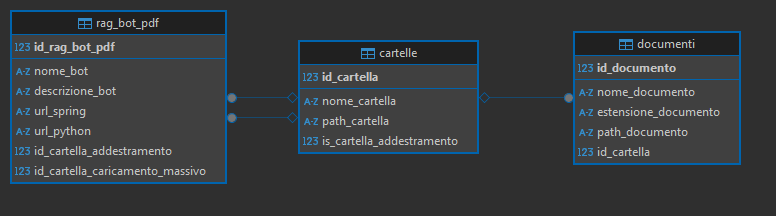
\includegraphics[width=0.8\textwidth, height=0.7\textheight, keepaspectratio]{immagini/Database bot.png}}

Il sistema di gestione dei dati per l'addestramento dei bot è organizzato secondo un modello relazionale composto da tre tabelle principali: \textbf{rag\scalebox{0.5}[1.0]{\_}bot\scalebox{0.5}[1.0]{\_}pdf}, \textbf{cartelle} e \textbf{documenti}. Di seguito viene descritto il ruolo e la struttura di ciascuna tabella, nonché le relazioni tra di esse. La tabella \textbf{rag\scalebox{0.5}[1.0]{\_}bot\scalebox{0.5}[1.0]{\_}pdf} contiene le configurazioni necessarie per ciascun bot. Qui di seguito vengono descritti i campi della tabella:

\begin{itemize}
\item \textbf{\textnormal{\lstinline|id_rag_bot_pdf|}}: Identificativo univoco del bot.
\item \textnormal{\lstinline|nome_bot|}: nome del bot
\item \textnormal{\lstinline|descrizione_bot|}: descrizione del bot
\item \textnormal{\lstinline|url_spring|}: URL utilizzato per l'integrazione con servizi esterni implementati in Spring.
\item \textnormal{\lstinline|url_python|}: URL utilizzato per l'integrazione con servizi esterni implementati in Python
\item \textnormal{\lstinline|id_cartella_addestramento|}: Riferimento alla cartella che contiene i file utilizzati per l'addestramento singolo del bot.
\item \textnormal{\lstinline|id_cartella_caricamento_massivo|}: Riferimento alla cartella utilizzata per la funzionalità di addestramento massivo.
\end{itemize}

La tabella \textbf{cartelle} è destinata alla gestione delle directory utilizzate per l'addestramento. Qui di seguito vengono descritti i campi della tabella:

\begin{itemize}
\item \textnormal{\lstinline|id_cartella|}: Identificativo univoco della cartella.
\item \textnormal{\lstinline|nome_cartella|}: Nome della cartella.
\item \textnormal{\lstinline|path_cartella|}: Percorso della cartella nel file system.
\item \textnormal{\lstinline|is_cartella_addestramento|}: Campo booleano che distingue tra:
	\begin{itemize}
	\item Cartella di addestramento singolo: Contiene i file già pronti per essere utilizzati nel processo di addestramento del bot.
	\item Cartella di addestramento massivo: Utilizzata esclusivamente per conservare file che verranno successivamente spostati nella cartella di addestramento singolo al 					momento dell’esecuzione della funzionalità di addestramento massivo.
	\end{itemize}
\end{itemize}

Il campo \textnormal{\lstinline|is_cartella_addestramento|} gioca un ruolo fondamentale nel distinguere le due tipologie di cartelle. La cartella di addestramento singolo è utilizzata direttamente nel processo di addestramento del bot, mentre la cartella di addestramento massivo funge da spazio temporaneo per conservare file che verranno successivamente caricati nella cartella di addestramento singolo. Questa distinzione consente di gestire in modo efficiente processi di addestramento su larga scala, garantendo la separazione tra i file temporanei e quelli effettivamente utilizzati dal bot.

La tabella documenti rappresenta i file utilizzati nel processo di addestramento. Qui di seguito vengono descritti i campi della tabella:
\begin{itemize}
\item \textnormal{\lstinline|id_documento|}: Identificativo univoco del documento.
\item \textnormal{\lstinline|nome_documento|}: Nome del file.
\item \textnormal{\lstinline|estensione_documento|}: Estensione o formato del file
\item \textnormal{\lstinline|path_documento|}: Percorso del file nel file system.
\item \textnormal{\lstinline|id_cartella|}: Collegamento alla cartella di appartenenza.
\end{itemize}

Le tre tabelle sono collegate per formare un sistema relazionale:
\begin{itemize}
\raggedright
\item La tabella \textnormal{\lstinline|rag_bot_pdf|} è associata alla tabella cartelle tramite i campi \textnormal{\lstinline|id_cartella_addestramento|} e \textnormal{\lstinline|id_cartella_caricamento_massivo|}, consentendo di associare un bot a due diverse directory: una per l'addestramento singolo e una per il caricamento massivo.
\item La tabella cartelle, a sua volta, è collegata alla tabella documenti tramite il campo \textnormal{\lstinline|id_cartella|}, che associa ogni documento a una specifica cartella.
\end{itemize}

Le altre tabelle del database sono destinate alla gestione del sistema sanitario in cui l'applicativo sarà utilizzato. Non fanno parte della gestione dei bot, ma possono essere adattate in base al contesto in cui i bot vengono creati. In futuro, si prevede comunque la possibilità di addestrare un bot utilizzando i dati presenti nel database e di sviluppare una memoria interna per il bot.

\subsection{Creazione dei microservizi REST}

Dopo aver creato i bot attraverso i relativi progetti in Python, come descritto nella sezione 2.1.1, si è proceduto allo sviluppo dei corrispondenti microservizi utilizzando Spring Boot, inclusa la realizzazione del microservizio System Management. I progetti relativi ai bot espongono endpoint specifici per consentire la comunicazione con gli altri componenti del sistema.

Il microservizio System Management adotta la metodologia Object-Relational Mapping (ORM) per mappare le entità del database su oggetti Java, agevolando la manipolazione dei dati e garantendo una stretta integrazione con la logica applicativa. Questo microservizio fornisce endpoint per operazioni essenziali come la registrazione, l'aggiornamento e l'eliminazione dei bot. Inoltre, include funzionalità per il caricamento dei file necessari e l'addestramento dei modelli, contribuendo a una gestione centralizzata ed efficace del ciclo di vita dei bot.

Un ruolo cruciale è svolto dal microservizio BFF (Backend for Frontend), progettato per fungere da ponte tra il front-end e gli altri microservizi. Al suo interno vengono memorizzati i file YAML, che descrivono le configurazioni e le specifiche di comunicazione tra i vari microservizi. Questo approccio semplifica il flusso dei dati, migliorando la modularità e riducendo la complessità nelle interazioni tra front-end e back-end. Il BFF consente al sistema di mantenere una chiara separazione delle responsabilità: i microservizi relativi ai bot e al System Management gestiscono rispettivamente le funzionalità core e la logica applicativa, mentre il BFF offre un'interfaccia ottimizzata per il front-end, migliorando l'esperienza utente e l'efficienza complessiva del sistema.

La configurazione dei path necessari per la comunicazione tra i microservizi è gestita dalla classe ExternalApiClientConfig, che centralizza e organizza i riferimenti ai percorsi esposti. Questo approccio garantisce una struttura modulare e facilmente manutenibile, permettendo di stabilire in modo chiaro e flessibile i percorsi per invocare le funzionalità offerte dai microservizi.

La gestione delle risposte derivanti dalle chiamate ai microservizi è affidata alla classe EsitoResponseErrorHandler, che si occupa di convertire e uniformare le risposte ricevute. Tali risposte vengono incapsulate in un oggetto generalizzato del tipo generico T, che include:

\begin{itemize}
\item un identificativo dell'operazione
\item una lista di messaggi che possono contenere informazioni, avvisi o errori,
\item il tipo di esito che specifica se l'operazione è andata a buon fine o meno.
\end{itemize}

Questa struttura consente una gestione uniforme delle risposte, migliorando la leggibilità e la manutenzione del codice. La generalizzazione introdotta dalla classe EsitoResponseErrorHandler offre inoltre maggiore flessibilità nel trattamento delle risposte, indipendentemente dal tipo specifico di payload restituito.

Per facilitare l'interazione con gli endpoint esposti dai microservizi, è stato integrato Swagger UI, un'interfaccia grafica intuitiva che permette agli sviluppatori e agli utenti di esplorare e testare gli endpoint. Swagger UI genera automaticamente documentazione interattiva basata su annotazioni presenti nel codice, rendendo l'accesso agli endpoint più immediato e agevole. Questa integrazione offre una soluzione user-friendly per inviare richieste e visualizzare risposte, eliminando la necessità di strumenti esterni o conoscenze approfondite dei dettagli di implementazione.

\bibliographystyle{plain}  
\bibliography{bibliografia}
\include{ringraziamenti}
\end{document}
